\chapter{الكيمياء الخضراء والعمليات الصناعية}\label{ch:b3:green-industrial}

كان الإيبوبروفين يُصنع قديمًا في ست خطوات تهدر من الكتلة أكثر مما
تحتفظ به: فأملاح الألومنيوم وكلوريد الصوديوم والإيثانول والأمونيا وحمض الأسيتيك
كانت تغادر المصنع مع كل كيلوغرام من الدواء. ومنذ سنة 1992 صار طريق حفزي
من ثلاث خطوات يحوّل معظم الذرات التي يستعملها إلى الناتج، ونواتجه الثانوية
لا تتعدى حمض الأسيتيك، الذي يُسترجع ويُباع. ويضع هذا الفصل أرقامًا على
مثل هذه المقارنات: \omterm{def:b3:green-industrial:atom-economy}{الاقتصاد الذري}، والعوامل E، \omterm{def:b3:green-industrial:pmi}{وكثافة الكتلة في العملية}؛ ثم
ينظر في المذيبات والطاقة \omterm{def:b3:green-industrial:lca}{وتقييم دورة الحياة}، وفي كيف جُعلت بعض أكبر
العمليات الكيميائية أنظف، وفيما تغيّره \omterm{def:b3:green-industrial:feedstock}{المواد الأولية المتجددة}
والإنزيمات.

\begin{recall}
قدّم المجلد المدرسي \omterm{def:b3:green-industrial:atom-economy}{الاقتصاد الذري} \omterm{def:b3:green-industrial:green-chemistry}{والكيمياء الخضراء}؛ وقدّم مجلد السنة الأولى
المردودات؛ ومجلد السنة الثانية المفاعلات، والتحويل، والانتقائية، وزمن
المكوث، والتحويل في مرور واحد، وإعادة التدوير والتنفيس، والارتفاع الأديباتي في درجة
الحرارة، والمحللات الكهربائية وخلايا الوقود. وعالجت \cref{ch:b3:surfaces-catalysis}
و\cref{ch:b3:homogeneous-catalysis} الحفز،
و\cref{ch:b3:total-synthesis} مقاييس الطريق التخليقي.
\end{recall}

\begin{omfigure}
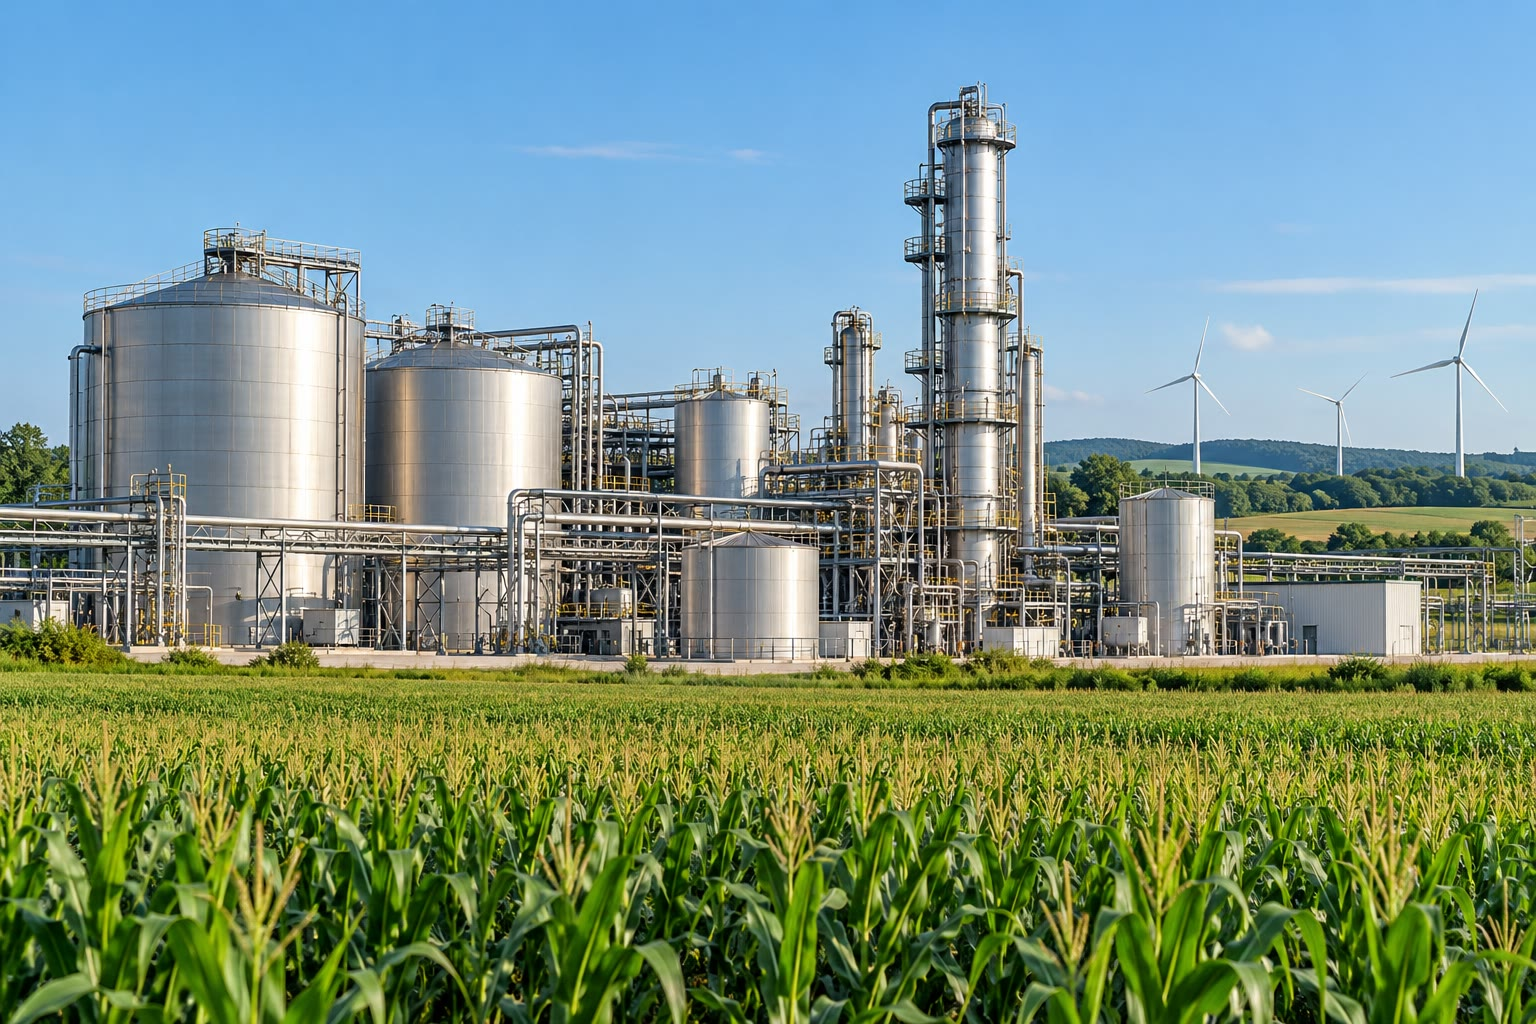
\includegraphics[width=0.58\linewidth]{images/book4/ai/b3-31-biorefinery.jpg}

{\small مصفاة حيوية: خزانات تخمير وعمود تقطير يحوّلان
المحاصيل والمخلفات إلى وقود ومواد كيميائية منصّية.}
\end{omfigure}

\section{قياس اخضرار العملية}

\begin{definition}[الكيمياء الخضراء]\label{def:b3:green-industrial:green-chemistry}
\emph{الكيمياء الخضراء}\index{كيمياء خضراء} هي تصميم المنتجات
والعمليات الكيميائية بحيث تقلل استعمال المواد الخطرة وتوليدها أو تزيلهما،
وتُلخَّص في اثني عشر مبدأ: منع النفايات، وتعظيم
\omterm{def:b3:green-industrial:atom-economy}{الاقتصاد الذري}، واستعمال مواد أقل خطرًا وصنعها، وتصميم منتجات أكثر أمانًا،
واستعمال مذيبات أكثر أمانًا، وتوفير الطاقة، واستعمال \omterm{def:b3:green-industrial:feedstock}{مواد أولية متجددة}، وتجنب المشتقات
غير الضرورية، وتفضيل الحفازات على الكواشف المستعملة بنسب ستوكيومترية، والتصميم من أجل
التحلل، والرصد في الزمن الحقيقي، واختيار كيمياء آمنة بطبيعتها.
\end{definition}

\begin{definition}[الاقتصاد الذري]\label{def:b3:green-industrial:atom-economy}
\emph{الاقتصاد الذري}\index{اقتصاد ذري} لتفاعل ما هو الكتلة المولية
للناتج المطلوب مقسومة على مجموع الكتل المولية لكل
المتفاعلات في المعادلة الموزونة، معبَّرًا عنه بنسبة مئوية.
\end{definition}

\begin{proposition}[الاقتصاد الذري بحسب صنف التفاعل]\label{prop:b3:green-industrial:ae-classes}
للإضافات وإعادات الترتيب \omterm{def:b3:green-industrial:atom-economy}{اقتصاد ذري} يساوي 100\,\%؛ وللاستبدالات
والحذف اقتصاد أقل.
\end{proposition}

\begin{proof}
في الإضافة، $\mathrm{A} + \mathrm{B} \to \mathrm{AB}$، أو في إعادة الترتيب، $\mathrm{A} \to \mathrm{A'}$، يحتوي الناتج الوحيد كل
ذرات المتفاعلات، فتساوي كتلته المولية مجموع كتلها المولية. أما
الاستبدال، $\mathrm{A{-}X} + \mathrm{Y} \to \mathrm{A{-}Y} + \mathrm{X}$، أو الحذف، $\mathrm{A} \to \mathrm{B} + \mathrm{C}$، فينتج
ناتجًا ثانيًا يحمل معه جزءًا من الكتلة.
\end{proof}

\begin{definition}[العامل E]\label{def:b3:green-industrial:e-factor}
\emph{العامل E}\index{عامل E} لعملية ما هو كتلة النفايات لكل وحدة كتلة من
الناتج. وفي العامل E الكامل تُحسب نفاياتٍ كلُّ المدخلات التي لا تنتهي في الناتج،
بما فيها المذيبات والماء؛ أما العامل E البسيط فيستثني المذيبات
والماء.
\end{definition}

\begin{definition}[كثافة الكتلة في العملية]\label{def:b3:green-industrial:pmi}
\emph{كثافة الكتلة في العملية}\index{كثافة الكتلة في العملية} (PMI) هي
الكتلة الكلية للمواد المُدخلة في عملية ما (المتفاعلات، والكواشف، والمذيبات،
والماء) لكل وحدة كتلة من الناتج.
\end{definition}

\begin{proposition}[كثافة الكتلة والعامل E]\label{prop:b3:green-industrial:pmi-e}
للحدود نفسها، $\mathrm{PMI} = E + 1$، حيث $E$ هو \omterm{def:b3:green-industrial:e-factor}{العامل E} الكامل.
\end{proposition}

\begin{proof}
بحفظ الكتلة، يغادر كل ما يدخل إما ناتجًا وإما نفايات:
$m_{\mathrm{in}} = m_{\mathrm{product}} + m_{\mathrm{waste}}$. وبالقسمة على $m_{\mathrm{product}}$ نحصل على $\mathrm{PMI} = 1 + E$.
\end{proof}

\begin{definition}[كفاءة كتلة التفاعل]\label{def:b3:green-industrial:rme}
\emph{كفاءة كتلة التفاعل}\index{كفاءة كتلة التفاعل} (RME) لتفاعل ما
هي كتلة الناتج المحصَّل مقسومة على الكتلة الكلية
للمتفاعلات المستعملة.
\end{definition}

\begin{proposition}[كفاءة كتلة التفاعل من المردود والاقتصاد الذري]\label{prop:b3:green-industrial:rme}
$\mathrm{RME} = \mathrm{AE} \times \text{المردود}/\mathrm{SF}$، حيث المعامل الستوكيومتري $\mathrm{SF} \ge 1$ هو كتلة
المتفاعلات المستعملة مقسومة على الكتلة التي تتطلبها المعادلة الموزونة.
\end{proposition}

\begin{proof}
من أجل مول واحد متوقع من الناتج، تتطلب المعادلة كتلة $\sum M_r$ من المتفاعلات
ويستعمل التشغيل $\mathrm{SF}\sum M_r$؛ ويعطي $\text{المردود} \times M_{\mathrm p}$ من الناتج. وبالقسمة:
$\mathrm{RME} = \text{المردود}\,M_{\mathrm p}/(\mathrm{SF}\sum M_r) = \mathrm{AE} \times \text{المردود}/\mathrm{SF}$.
\end{proof}

\begin{method}[حساب مقاييس طريق تخليقي]\label{met:b3:green-industrial:metrics}
\begin{enumerate}
  \item اكتب المعادلة الموزونة لكل خطوة واحسب \omterm{def:b3:green-industrial:atom-economy}{الاقتصاد الذري}
        للطريق من كل المتفاعلات التي تدخله.
  \item من سجل الدفعة، اجمع كتل كل ما شُحن (المتفاعلات،
        والكواشف، والمذيبات، والماء، ومواد المعالجة): كثافة الكتلة تساوي مجموع المدخلات مقسومًا على كتلة الناتج.
  \item $E = \mathrm{PMI} - 1$؛ اطرح التيارات المسترجعة والمعاد استعمالها إن كانت داخل
        الحدود، وصرّح بذلك.
  \item \omterm{def:b3:green-industrial:rme}{كفاءة كتلة التفاعل} لكل خطوة: الناتج مقسومًا على المتفاعلات، لتجد أين تضيع المادة
        (مردود منخفض، أو فائض من الكاشف، أو \omterm{def:b3:green-industrial:atom-economy}{اقتصاد ذري} ضعيف).
\end{enumerate}
\end{method}

\begin{omfigure}
\begin{tikzpicture}
\begin{axis}[name=a, width=0.48\linewidth, height=5.4cm, ybar, bar width=14pt, ymin=0, ymax=110,
  xtick={1,2,3,4}, xticklabels={{\foreignlanguage{arabic}{إيبوبروفين، 6 خطوات}}, {\foreignlanguage{arabic}{إيبوبروفين، 3 خطوات}}, {\foreignlanguage{arabic}{أكسيد الإيثيلين، كلوروهيدرين}}, {\foreignlanguage{arabic}{أكسيد الإيثيلين، مباشر}}},
  x tick label style={font=\scriptsize, rotate=25, anchor=north east}, ylabel={\foreignlanguage{arabic}{الاقتصاد الذري \babelsublr{/ \%}}},
  axis lines=left, tick label style={font=\scriptsize}, label style={font=\small},
  nodes near coords, nodes near coords style={font=\scriptsize, /pgf/number format/fixed, /pgf/number format/precision=0},
  enlarge x limits=0.18]
\addplot[fill=omMeth!55, draw=omMeth] table[x=i, y=AE] {figdata/out/bachelor-3-green-metrics.dat};
\end{axis}
\begin{axis}[at={(a.east)}, anchor=west, xshift=1.4cm, width=0.48\linewidth, height=5.4cm, ybar, bar width=14pt, ymin=0, ymax=3.4,
  xtick={1,2,3,4}, xticklabels={{\foreignlanguage{arabic}{إيبوبروفين، 6 خطوات}}, {\foreignlanguage{arabic}{إيبوبروفين، 3 خطوات}}, {\foreignlanguage{arabic}{أكسيد الإيثيلين، كلوروهيدرين}}, {\foreignlanguage{arabic}{أكسيد الإيثيلين، مباشر}}},
  x tick label style={font=\scriptsize, rotate=25, anchor=north east}, ylabel={\foreignlanguage{arabic}{أدنى عامل E}},
  axis lines=left, tick label style={font=\scriptsize}, label style={font=\small},
  nodes near coords, nodes near coords style={font=\scriptsize, /pgf/number format/fixed, /pgf/number format/precision=2},
  enlarge x limits=0.18]
\addplot[fill=omThm!45, draw=omThm] table[x=i, y=Emin] {figdata/out/bachelor-3-green-metrics.dat};
\end{axis}
\end{tikzpicture}

{\small \omterm{def:b3:green-industrial:atom-economy}{الاقتصاد الذري} لطريقين إلى الإيبوبروفين وطريقين إلى أكسيد الإيثيلين،
وأصغر العوامل E التي يسمحان بها (كل المردودات 100\,\%، دون مذيب):
$E_{\min} = (1 - \mathrm{AE})/\mathrm{AE}$. أما العوامل E الحقيقية، مع مردودات دون 100\,\% وكواشف فائضة
ومذيبات، فأكبر.}
\end{omfigure}

\section{المذيبات والطاقة}

المذيبات هي عادة الجزء الأكبر من كتلة عملية في الكيمياء الدقيقة أو
الصيدلانية. وترتّبها أدلة اختيار المذيبات بحسب معايير السلامة والصحة
والبيئة: فالماء والإيثانول وأسيتات الإيثيل و2-ميثيل رباعي هيدروفوران
والأنيسول موصى بها؛ أما ثنائي كلوروميثان والكلوروفورم والبنزين والهكسان
وثنائي ميثيل فورماميد و1،4-ديوكسان فيجب تجنبها أو هي محظورة. والماء،
وثنائي أكسيد الكربون فوق الحرج (الذي يذيب المركبات غير القطبية ولا يترك
أثرًا حين يُخفَّف الضغط) والتفاعلات دون مذيب تزيل
المشكلة من مصدرها.

\begin{method}[استعمال دليل اختيار المذيبات]\label{met:b3:green-industrial:solvent-choice}
\begin{enumerate}
  \item عدّد ما يجب أن يفعله المذيب: أن يذيب المتفاعلات، ويصمد أمام الكواشف،
        ويغلي عند درجة حرارة مناسبة، وينفصل عن الماء عند المعالجة.
  \item اختر من الصنف الموصى به أولًا؛ وتحقق من عبارات الخطر الخاصة به.
  \item إن لزم مذيب إشكالي، فابحث عن مذيب موصى به يؤدي
        الوظيفة نفسها (2-ميثيل رباعي هيدروفوران مكان ثنائي كلوروميثان أو THF في
        الاستخلاصات، وأسيتات الإيثيل والهبتان مكان الهكسان في الكروماتوغرافيا).
  \item خطط لاسترجاعه بالتقطير، واحسب ما يضيع منه في \omterm{def:b3:green-industrial:e-factor}{العامل E}.
\end{enumerate}
\end{method}

\begin{definition}[تكثيف العمليات]\label{def:b3:green-industrial:intensification}
\emph{تكثيف العمليات}\index{تكثيف العمليات} هو
إعادة تصميم المعدات وظروف التشغيل لجعل العملية أصغر بكثير، أو
أكثر أمانًا أو كفاءة: مفاعلات التدفق المستمر ذات الأحجام الصغيرة
ومساحات التبادل الحراري الكبيرة، والتقطير التفاعلي، والتسخين بالموجات الدقيقة.
\end{definition}

في مفاعل التدفق لا يوجد في أي لحظة إلا حجم صغير من وسيط
خطر، وتُنزع الحرارة أسرع بكثير مما في وعاء دفعات كبير؛ فالتفاعلات
التي كانت ستنفلت في خزان يمكن إجراؤها عند درجات حرارة وتراكيز
أعلى. وتحل الحفازات محل الكواشف المستعملة بنسب ستوكيومترية، فتوفّر
الكاشف والنفايات التي يصير إليها معًا: فقد استعملت أسيلة فريدل--كرافتس في طريق
الإيبوبروفين القديم كلوريد الألومنيوم بكمية ستوكيومترية تُتلف عند
المعالجة؛ أما الطريق الجديد فيستعمل فلوريد الهيدروجين حفازًا ومذيبًا،
يُسترجع ويُعاد استعماله.

\section{التفكير بدورة الحياة}

\begin{definition}[تقييم دورة الحياة]\label{def:b3:green-industrial:lca}
\emph{تقييم دورة الحياة}\index{تقييم دورة الحياة} (LCA) يقدّر
الآثار البيئية لمنتج على امتداد حياته، من استخراج المواد الخام
إلى التخلص منه. ويُعبَّر عنه لكل \emph{وحدة وظيفية}\index{وحدة وظيفية}،
أي الخدمة المقدَّمة (مثل غسلة واحدة لحمولة من الغسيل)، داخل
\emph{حدود النظام}\index{حدود النظام} التي تحدد أي العمليات
مشمولة. أما \emph{التقييم من المهد إلى البوابة}\index{تقييم من المهد إلى البوابة}
فيتوقف حين يغادر المنتج المصنع.
\end{definition}

\begin{omfigure}
\begin{tikzpicture}[font=\scriptsize, >=Stealth,
  box/.style={draw, rounded corners, fill=omDef!10, align=center, minimum height=8mm, inner sep=3pt}]
  \node[box] (r) at (0,0) {\foreignlanguage{arabic}{استخراج}\\ \foreignlanguage{arabic}{المواد الخام}};
  \node[box] (p) at (2.6,0) {\foreignlanguage{arabic}{الإنتاج}\\ \foreignlanguage{arabic}{الكيميائي}};
  \node[box] (f) at (5.2,0) {\foreignlanguage{arabic}{التركيب،}\\ \foreignlanguage{arabic}{التعبئة}};
  \node[box] (u) at (7.8,0) {\foreignlanguage{arabic}{الاستعمال}};
  \node[box] (e) at (10.2,0) {\foreignlanguage{arabic}{نهاية الحياة:}\\ \foreignlanguage{arabic}{تدوير، تخلّص}};
  \foreach \a/\b in {r/p, p/f, f/u, u/e} \draw[->, thick] (\a) -- (\b);
  \draw[omThm, thick, dashed, rounded corners] (-1.1,-0.75) rectangle (3.75,0.75);
  \node[omThm, anchor=north] at (1.3,-0.8) {\foreignlanguage{arabic}{حدود من المهد إلى البوابة}};
  \draw[omMeth, thick, dashed, rounded corners] (-1.25,-1.35) rectangle (11.5,0.95);
  \node[omMeth, anchor=north] at (5.1,-1.4) {\foreignlanguage{arabic}{حدود من المهد إلى اللحد}};
  \node[anchor=south] at (5.1,1.0) {\foreignlanguage{arabic}{المدخلات: مواد، طاقة، ماء \quad المخرجات: منتج، انبعاثات، نفايات}};
\end{tikzpicture}

{\small مراحل حياة منتج وحدودا نظام اثنتان. تُجرد المدخلات والمخرجات
لكل عملية داخل الحدود وتُحوَّل إلى فئات
أثر (تغير المناخ، والتحمض، واستعمال الماء، والسمية\dots) لكل
\omterm{def:b3:green-industrial:lca}{وحدة وظيفية}.}
\end{omfigure}

\begin{definition}[البصمة الكربونية]\label{def:b3:green-industrial:carbon-footprint}
\emph{البصمة الكربونية}\index{بصمة كربونية} لمنتج ما هي
انبعاثه من غازات الدفيئة على امتداد دورة حياته، معبَّرًا عنه بكتلة ثنائي أكسيد الكربون
ذات أثر الاحترار نفسه.
\end{definition}

\begin{method}[إعداد تقييم مقارن لدورة الحياة]\label{met:b3:green-industrial:lca}
\begin{enumerate}
  \item حدّد الهدف \omterm{def:b3:green-industrial:lca}{والوحدة الوظيفية}: قارن ما يقدّم الخدمة
        نفسها، لا الكتلة نفسها.
  \item ارسم \omterm{def:b3:green-industrial:lca}{حدود النظام} نفسها للخيارين كليهما.
  \item اجرد مدخلات كل عملية داخلها ومخرجاتها، مع مصادر
        البيانات وتواريخها.
  \item حوّلها إلى فئات أثر، ثم ابحث عن المقايضات (كربون أقل لكن
        ماء أكثر) واختبر مدى حساسية الاستنتاج للبيانات.
\end{enumerate}
\end{method}

\section{العمليات الكبرى وتحسينها}

\begin{proposition}[ثنائي أكسيد الكربون من الأمونيا]\label{prop:b3:green-industrial:smr}
صنع الأمونيا بهيدروجين مأخوذ من إصلاح الميثان بالبخار يطلق، من
المادة الأولية وحدها، $3/8$ مول من $\ce{CO2}$ لكل مول من $\ce{NH3}$: أي نحو \qty{0.97}{t} من $\ce{CO2}$ لكل طن من الأمونيا.
\end{proposition}

\begin{proof}
الإصلاح متبوعًا بتفاعل إزاحة الماء--الغاز هو إجمالًا $\ce{CH4 + 2H2O -> CO2 + 4H2}$. والتخليق
هو $\ce{N2 + 3H2 -> 2NH3}$: فمولا الأمونيا يحتاجان إلى ثلاثة مولات من الهيدروجين، أي $3/4$ مول من
الميثان و$3/4$ مول من $\ce{CO2}$؛ ولكل مول من الأمونيا $3/8$. والطن من الأمونيا
(\qty{17.0}{g/mol}) يساوي $\qty{5.88e4}{mol}$، فيعطي $\qty{2.21e4}{mol} \times \qty{44.0}{g/mol} = \qty{0.97}{t}$ من $\ce{CO2}$. وحرق الميثان
لتوفير حرارة الإصلاح يضيف المزيد.
\end{proof}

% ledger: nh3:world-2024
تُعد مصانع الأمونيا، التي تنتج نحو 150 مليون طن من النيتروجين سنويًا، من
أكبر المصادر المنفردة لثنائي أكسيد الكربون الصناعي؛ والهيدروجين المنتَج
بالتحليل الكهربائي بكهرباء منخفضة الكربون، أو احتجاز الكربون عند وحدة الإصلاح،
هما سبيلا خفضه. أما حلقة الأمونيا نفسها، بتحويلها المنخفض في المرور
الواحد، وإعادة تدوير الغاز غير المتفاعل وتنفيس الأرغون والميثان اللذين
كانا سيتراكمان لولا ذلك، فهي كفوءة أصلًا.

\begin{omfigure}
\begin{tikzpicture}[font=\scriptsize, >=Stealth,
  box/.style={draw, rounded corners, fill=omMeth!10, align=center, minimum height=8mm, inner sep=3pt}]
  \node[box] (m) at (0,0) {\foreignlanguage{arabic}{خلّاط}};
  \node[box] (c) at (2.6,0) {\foreignlanguage{arabic}{ضاغط}};
  \node[box] (r) at (5.2,0) {\foreignlanguage{arabic}{مُحوِّل}\\ \foreignlanguage{arabic}{بحفاز الحديد}};
  \node[box] (s) at (8.0,0) {\foreignlanguage{arabic}{مكثف،}\\ \foreignlanguage{arabic}{فاصل}};
  \draw[->, thick] (-1.8,0) -- (m) node[pos=0, left, align=right] {$\ce{N2 + 3H2}$\\ \foreignlanguage{arabic}{غاز التعويض}};
  \draw[->, thick] (m) -- (c); \draw[->, thick] (c) -- (r); \draw[->, thick] (r) -- (s);
  \draw[->, thick] (s) -- ++(0,-1.2) node[below] {\foreignlanguage{arabic}{$\ce{NH3}$ سائلة}};
  \draw[->, thick] (s.north) -- ++(0,0.8) -| node[pos=0.25, above] {\foreignlanguage{arabic}{إعادة تدوير الغاز غير المتفاعل}} (m.north);
  \draw[->, thick, omThm] ($(s.north)+(0,0.8)$) -- ++(1.6,0) node[right] {\foreignlanguage{arabic}{تنفيس: الأرغون و$\ce{CH4}$}};
\end{tikzpicture}

{\small حلقة تخليق الأمونيا: يُمزج الغاز الطازج بالغاز المعاد تدويره،
ويُضغط ويُمرَّر على الحفاز؛ وتُكثَّف الأمونيا وتُفصل، ويعود الغاز
غير المتفاعل، ويزيل تيار تنفيس صغير الغازات الخاملة التي كانت
ستتراكم لولا ذلك.}
\end{omfigure}

وتُظهر العمليات الكبرى الأخرى الدروس نفسها. فعملية التلامس لإنتاج حمض
الكبريتيك ناشرة للحرارة إلى حد أن المصنع الحديث يصدّر البخار والكهرباء.
وكان أكسيد الإيثيلين يُصنع أولًا عبر كلوروهيدرين الإيثيلين، مع كلوريد
الكالسيوم نفاياتٍ؛ ثم حلت محله الأكسدة المباشرة للإيثيلين بالأكسجين على الفضة، وهي
إضافة \omterm{def:b3:green-industrial:atom-economy}{باقتصاد ذري} 100\,\%، مقابل احتراق جزء من الإيثيلين إلى
ثنائي أكسيد الكربون. ويُصنع أكسيد البروبيلين اليوم أيضًا بفوق أكسيد الهيدروجين على
حفاز زيوليتي بالتيتانيوم، والماء ناتجه الثانوي الوحيد. أما حمض الأديبيك،
المصنوع بأكسدة الهكسانول الحلقي والهكسانون الحلقي بحمض النتريك، فيطلق
أكسيد النيتروز، وهو غاز دفيئة قوي، تُتلفه المصانع اليوم حفزيًا.

\section{المواد الأولية المتجددة والحفز الحيوي}

\begin{definition}[المواد الأولية المتجددة]\label{def:b3:green-industrial:feedstock}
\emph{المادة الأولية المتجددة}\index{مادة أولية متجددة} مادة خام
تتجدد على مقياس زمني بشري، مثل الكتلة الحيوية النباتية. و\emph{الجزيء
المنصّي}\index{جزيء منصّي} مركب بسيط يُصنع منها بكميات
كبيرة ويُحوَّل إلى منتجات كثيرة: الإيثانول، وحمض اللبنيك، وحمض السكسينيك،
والغليسرول، وحمض الليفولينيك، والفورفورال، و5-(هيدروكسي ميثيل)فورفورال.
\end{definition}

\begin{definition}[الحفز الحيوي]\label{def:b3:green-industrial:biocatalysis}
\emph{الحفز الحيوي}\index{حفز حيوي} هو استعمال الإنزيمات، معزولةً أو داخل
الخلايا، حفازاتٍ للتحولات الكيميائية.
\end{definition}

تعمل الإنزيمات في الماء قرب درجة حرارة الغرفة بانتقائية بالغة الدقة، 
ويكيّفها التطور الموجَّه اليوم مع ركائز غير طبيعية: فقد حل \omterm{def:b3:complex-kinetics:enzyme}{إنزيم} ناقل للأمين
طُوِّر لهذا الغرض محل هدرجة لاتناظرية محفَّزة بالروديوم
في صنع دواء السكري سيتاغليبتين، وتصنع إنزيمات مختزلة للكيتونات كثيرًا من
الكحولات الكيرالية. وثنائي أكسيد الكربون نفسه مادة أولية: فمنه ومن الأمونيا
تُصنع اليوريا، ومنه ومن الهيدروجين يُصنع الميثانول. ويمكن إعادة البولي إيثيلين تيريفثالات
إلى مونومراته بإزالة البلمرة بالتحلل الغليكولي أو بالتحلل الميثانولي، أو
بإنزيمات مهندَسة، ثم بلمرتها من جديد.

\begin{inthelab}[استبدال ثنائي كلوروميثان في المعالجة]
ناتج كان يُستخلص من الماء بثنائي كلوروميثان يُستخلص
الآن بالمركب 2-ميثيل رباعي هيدروفوران: فهو مصنوع من الكتلة الحيوية، وينفصل
عن الماء انفصالًا نظيفًا (فهو لا يمتزج به إلا جزئيًا)، ويكوّن الطبقة العليا لا
السفلى، وهذا يغيّر ترتيب عمليات قمع الفصل. ثم تُجفَّف
الطبقات العضوية، ويُقطَّر المذيب تحت ضغط مخفَّض
ويُجمع لإعادة استعماله.
\end{inthelab}

\begin{safety}{\ghs[0.62cm]{GHS02}\ghs[0.62cm]{GHS04}\ghs[0.62cm]{GHS06}\ghs[0.62cm]{GHS08}}
% ledger: ghs4:EO, ghs:CH2Cl2, ghs4:2MeTHF
أكسيد الإيثيلين: غاز شديد الاشتعال تحت الضغط، سام بالاستنشاق، وقد
يسبب السرطان والعيوب الوراثية؛ ولا وجود له إلا في الأنظمة الصناعية المغلقة
ووحدات التعقيم. وثنائي كلوروميثان مشتبه في أنه مسرطن، 
و2-ميثيل رباعي هيدروفوران قابل للاشتعال وأكّال للعينين: فالمذيب الأكثر اخضرارًا
ليس مذيبًا عديم الضرر.
\end{safety}

\begin{history}[اثنا عشر مبدأ ورقم واحد]
نشر بول أناستاس وجون وارنر المبادئ الاثني عشر \omterm{def:b3:green-industrial:green-chemistry}{للكيمياء
الخضراء} سنة 1998. وأدخل روجر شيلدون \omterm{def:b3:green-industrial:e-factor}{العامل E} سنة 1992، ملاحظًا أن
صناعتي الكيمياء الدقيقة والأدوية، وإن صغرت حمولتهما بالأطنان،
تنتجان نفايات لكل كيلوغرام من الناتج أكثر بكثير مما تنتجه كيمياء السلع الكبرى. وصارت
عملية الإيبوبروفين ذات الخطوات الثلاث، التي بدأت سنة 1992، من أوائل
الأمثلة على النهج الجديد.
\end{history}

\section{تمارين}

\begin{exercise}[$\star$]\label{exo:b3:green-industrial:1}
احسب \omterm{def:b3:green-industrial:atom-economy}{الاقتصاد الذري} لتفاعل ديلز--ألدر بين البوتاديين والإيثين، ولأسترة
حمض الأسيتيك بالإيثانول، ولتفاعل فيتيغ بين
البنزالدهيد و$\ce{Ph3P=CH2}$ (الذي يعطي الستايرين وأكسيد ثلاثي فينيل الفوسفين).
\end{exercise}

\begin{exercise}[$\star$]\label{exo:b3:green-industrial:2}
تستعمل دفعة 120 kg من المواد (متفاعلات ومذيبات وماء) وتعطي 8.0 kg من
الناتج. احسب \omterm{def:b3:green-industrial:pmi}{كثافة الكتلة في العملية} \omterm{def:b3:green-industrial:e-factor}{والعامل E} الكامل.
\end{exercise}

\begin{exercise}[$\star$]\label{exo:b3:green-industrial:3}
اختر \omterm{def:b3:green-industrial:lca}{وحدة وظيفية} لمقارنة منظّفي غسيل، وقل لماذا
تكون «كيلوغرام واحد من المسحوق» اختيارًا سيئًا.
\end{exercise}

\begin{exercise}[$\star$]\label{exo:b3:green-industrial:4}
اقترح بدائل أكثر اخضرارًا لثنائي كلوروميثان في الاستخلاص، وللهكسان في
الكروماتوغرافيا، ولثنائي ميثيل فورماميد في اقتران تكوين الأميد.
\end{exercise}

\begin{exercise}[$\star\star$]\label{exo:b3:green-industrial:5}
أسترة 60.0 g من حمض الأسيتيك مع 92.0 g من الإيثانول (ضعف
الكمية الستوكيومترية) تعطي 70.4 g من أسيتات الإيثيل. احسب المردود، \omterm{def:b3:green-industrial:atom-economy}{والاقتصاد
الذري}، والمعامل الستوكيومتري \omterm{def:b3:green-industrial:rme}{وكفاءة كتلة التفاعل}، وتحقق من العلاقة
بينها.
\end{exercise}

\begin{exercise}[$\star\star$]\label{exo:b3:green-industrial:6}
احسب \omterm{def:b3:green-industrial:atom-economy}{الاقتصاد الذري} لطريقي الكلوروهيدرين والأكسدة المباشرة إلى
أكسيد الإيثيلين، وكتلة كلوريد الكالسيوم الناتجة لكل طن من أكسيد الإيثيلين
بالطريق الأول.
\end{exercise}

\begin{exercise}[$\star\star$]\label{exo:b3:green-industrial:7}
تحقق من كتلة $\ce{CO2}$ لكل طن من الأمونيا الواردة في الفصل، واحسب كتلة $\ce{CO2}$ لكل طن من
الهيدروجين المصنوع بإصلاح الميثان بالبخار.
\end{exercise}

\begin{exercise}[$\star\star$]\label{exo:b3:green-industrial:8}
احسب أدنى طاقة كهربائية، بالكيلوواط ساعة، لصنع كيلوغرام واحد من الهيدروجين
بالتحليل الكهربائي للماء السائل عند \qty{25}{\celsius}، انطلاقًا من $\Delta_rG^\circ$، والطاقة انطلاقًا من $\Delta_rH^\circ$.
\end{exercise}

\begin{exercise}[$\star\star$]\label{exo:b3:green-industrial:9}
إذا تكوّن مول واحد من $\ce{N2O}$ لكل مول من حمض الأديبيك ($\ce{C6H10O4}$) وكانت قدرة الاحترار
العالمي للمركب $\ce{N2O}$ تساوي 273 (من معطيات التمرين)، فاحسب كتلة $\ce{N2O}$ ومكافئ $\ce{CO2}$
لكل طن من حمض الأديبيك دون معالجة للانبعاثات.
\end{exercise}

\begin{exercise}[$\star\star\star$]\label{exo:b3:green-industrial:10}
بيّن أن \omterm{def:b3:green-industrial:rme}{كفاءة كتلة التفاعل} الإجمالية لتسلسل من الخطوات ليست جداء كفاءات
الخطوات حين يُعاد تدوير الكواشف الفائضة، وفسّر كيف تغيّر إعادة التدوير
\omterm{def:b3:green-industrial:e-factor}{العامل E}.
\end{exercise}

\begin{exercise}[$\star\star\star$]\label{exo:b3:green-industrial:11}
يخفض تحسين في العملية المذيب في إحدى الخطوات من 20 L إلى 5 L لكل كيلوغرام من
الناتج (كثافة المذيب \qty{0.80}{kg/L}، ويُسترجع 90\,\% منه بالتقطير قبل التحسين وبعده؛ من معطيات
التمرين). احسب التغير في \omterm{def:b3:green-industrial:e-factor}{العامل E} الكامل.
\end{exercise}

\begin{exercise}[$\star\star\star$]\label{exo:b3:green-industrial:12}
لطريق حيوي المصدر إلى مونومر \omterm{def:b3:green-industrial:carbon-footprint}{بصمة كربونية} أدنى، لكنه يحتاج إلى أرض
وماء أكثر مما يحتاج إليه الطريق البتروكيميائي. كيف يعرض تقييم مقارن لدورة الحياة ذلك،
وما الذي تحتاج إليه للمفاضلة بينهما؟
\end{exercise}

\section{مسألة: الإيبوبروفين، ست خطوات أم ثلاث؟}

\begin{problem}[{مسألة نهاية الأسبوع --- الإيبوبروفين، ست خطوات أم ثلاث: الاقتصاد
الذري للطريقين، وعواملهما E، والحفازات التي تصنع
الفرق، والنفايات المتجنَّبة في سنة}]
\label{pb:b3:green-industrial:1}
% ledger: aw:C, aw:H, aw:O, aw:Cl, aw:Na, aw:N
معطيات المسألة، لكل طن من الإيبوبروفين. الطريق ذو الخطوات الثلاث: 0.71 طن من
الإيزوبوتيل بنزين، و0.55 طن من أنهيدريد الأسيتيك، و0.010 طن من الهيدروجين، و0.14 طن من أول أكسيد
الكربون، و0.05 طن من المذيب والحفاز المفقودين؛ ويُسترجع 0.31 طن من حمض الأسيتيك
ويُباع. الطريق ذو الخطوات الست: 2.0 طن من الكواشف و1.5 طن من المذيبات والمواد
المساعدة غير المسترجعة. ويصنع مصنع 3000 طن من الإيبوبروفين سنويًا.

\medskip\noindent\textbf{الجزء الأول --- \omterm{def:b3:green-industrial:atom-economy}{الاقتصاد الذري}.}
\begin{enumerate}
  \item اكتب الخطوات الثلاث للطريق الحفزي.
  \item اكتب معادلته الإجمالية.
  \item احسب الكتل المولية المعنية \omterm{def:b3:green-industrial:atom-economy}{والاقتصاد الذري}.
  \item عدّد متفاعلات الطريق ذي الخطوات الست (أسيلة فريدل--كرافتس، وتكاثف
        دارزنس مع كلورو أسيتات الإيثيل وإيثوكسيد الصوديوم، والحلمأة
        ونزع الكربوكسيل، وتكوين الأوكسيم، ونزع الماء إلى النتريل، والحلمأة).
  \item احسب اقتصاده الذري من مجموع كتلها المولية (مع جزيئين من
        الماء).
  \item ما النواتج الثانوية التي تغادر الطريق القديم؟
\end{enumerate}

\medskip\noindent\textbf{الجزء الثاني --- العوامل E.}
\begin{enumerate}[resume]
  \item احسب الكتلة المُدخلة في الطريق الجديد لكل طن من الناتج.
  \item احسب كثافة الكتلة فيه وعامله E الكامل، مع احتساب حمض الأسيتيك نفايات.
  \item احسب \omterm{def:b3:green-industrial:e-factor}{العامل E} إذا احتُسب حمض الأسيتيك المسترجع ناتجًا.
  \item احسب كثافة الكتلة \omterm{def:b3:green-industrial:e-factor}{والعامل E} للطريق القديم.
  \item لماذا يكون \omterm{def:b3:green-industrial:e-factor}{العامل E} الحقيقي أكبر من $(1 - \mathrm{AE})/\mathrm{AE}$؟
  \item أي المبادئ الاثني عشر توضحها هذه الفروق؟
\end{enumerate}

\medskip\noindent\textbf{الجزء الثالث --- الحفازات.}
\begin{enumerate}[resume]
  \item ما الذي يحل فلوريد الهيدروجين محله في الأسيلة، ولماذا يهم ذلك؟
  \item ما الذي يحفز هدرجة الكيتون إلى الكحول؟
  \item ما الذي يحفز \omterm{def:b3:homogeneous-catalysis:carbonylation}{كربونلة} الكحول، وإلى كيمياء أي فصل
        تنتمي؟
  \item لماذا يكون حمض الأسيتيك ناتجًا ثانويًا في الطريقين كليهما؟
  \item ما المخاطر التي يأتي بها الطريق الجديد، وكيف تُدار؟
  \item لماذا تعني الخطوات الأقل طاقة أقل أيضًا؟
\end{enumerate}

\medskip\noindent\textbf{الجزء الرابع --- سنة كاملة.}
\begin{enumerate}[resume]
  \item احسب نفايات الطريق القديم للإنتاج السنوي للمصنع.
  \item احسب نفايات الطريق الجديد (مع بيع حمض الأسيتيك).
  \item احسب النفايات المتجنَّبة سنويًا.
  \item هل يعني \omterm{def:b3:green-industrial:e-factor}{العامل E} الأدنى دائمًا أثرًا بيئيًا أدنى؟
  \item ما الذي يضيفه \omterm{def:b3:green-industrial:lca}{تقييم دورة الحياة}؟
  \item اذكر النتيجة: \omterm{def:b3:green-industrial:atom-economy}{الاقتصاد الذري} للطريق ذي الخطوات الثلاث.
\end{enumerate}
\end{problem}
